\documentclass[12pt]{article}
\usepackage{amsmath, amssymb}
\usepackage{geometry}[margin=10mm]
\usepackage{tikz-cd}
\usepackage{tikz}
\usepackage{bm}
\usepackage{mathrsfs}
\usepackage{bbm}
\usepackage[colorlinks=true, linkcolor=black, urlcolor=black, citecolor=black]{hyperref}
\geometry{margin=1in}
\newcommand{\dottoeq}[2]{%
    \noindent\makebox[0pt][l]{#1}%
    \hfill%
    \tikz[baseline] \draw[dotted] (0,.5ex) -- (2, .5ex);%
    \hspace{0.2em}(\ref{#2})%
}
\title{\textbf{Linear Algebra (Part 009)}\\[1ex]
\large Matrix Rrepresentation of Linear Mappings}
\author{Dr.Kapil\\\href{mailto:kapil@nitkkr.ac.in}{kapil@nitkkr.ac.in}\\Department of Computer Applications\\NIT Kurukshetra}
\begin{document}
\maketitle
From the previous part, we know all $n$-dimensional vector spaces are isomorphic to one another and hence with $\mathbb{R}^n$.
\newline
Let $\{\vec{b}_1, \dots, \vec{b}_n\}$ be the basis vectors for the given vector space.
\\
$B$ is an ordered basis: 
$
B_1 = [\vec{b}_1, \vec{b}_2, \dots, \vec{b}_n]
$
\\
Unordered basis set: 
$
{B_2} = \{\vec{b}_1, \vec{b}_2, \dots, \vec{b}_n\}
$\\
And the matrix with basis vectors in columns:
$
{B_3} = [\vec{b}_1\; \vec{b}_2\; \cdots\; \vec{b}_n]
$
\newline

{Definition \textit{(Coordinates)}}: Let $V$ be a vector space and $B = (\vec{b}_1, \dots, \vec{b}_n)$ an ordered basis of $V$.
For any $\vec{x} \in V$, it can be written as a unique linear combination of the basis vectors. Therefore,
$$
\vec{x} = \alpha_1 \vec{b}_1 + \alpha_2 \vec{b}_2 + \cdots + \alpha_n \vec{b}_n.
$$

$\therefore$ coordinates of $\vec{x}$ with respect to $B$ is $(\alpha_1, \alpha_2, \dots, \alpha_n)$.
\\
\newline
\textbf{Canonical / Standard Basis}

Example in 3D:

$$
\left\{
\begin{bmatrix} 1 \\ 0 \\ 0 \end{bmatrix},
\begin{bmatrix} 0 \\ 1 \\ 0 \end{bmatrix},
\begin{bmatrix} 0 \\ 0 \\ 1 \end{bmatrix}
\right\}
\quad \text{(denoted as } \vec{e}_1, \vec{e}_2, \vec{e}_3\text{)}
$$

Although generally we take our basis vectors as above, any basis vector set can provide a valid coordinate system.

Let $(2, 3)$ be a point in the standard basis of $\mathbb{R}^2$, i.e.,

$$
2 \times \begin{bmatrix} 1 \\ 0 \end{bmatrix}
+ 3 \times \begin{bmatrix} 0 \\ 1 \end{bmatrix}
= \begin{bmatrix} 2 \\ 3 \end{bmatrix}
$$

*Can you find the coordinates of this point in $B$ ?  
$$
B = \left\{
\begin{bmatrix} 1 \\ 1 \end{bmatrix},
\begin{bmatrix} 1 \\ 0 \end{bmatrix}
\right\}
$$
What is $\alpha, \beta$ such that:
$
\alpha \begin{bmatrix} 1 \\ 1 \end{bmatrix}
+ \beta \begin{bmatrix} 1 \\ 0 \end{bmatrix}
= \begin{bmatrix} 2 \\ 3 \end{bmatrix}
$\\
\newline
After solving, you get: $\alpha = 3$, $\beta = -1$.\\
\newline
Therefore, for the basis 
$
\left\{
\begin{bmatrix} 1 \\ 1 \end{bmatrix},
\begin{bmatrix} 1 \\ 0 \end{bmatrix}
\right\}
\quad \text{the coordinates of the point } \begin{bmatrix} 2 \\ 3 \end{bmatrix} \text{ are } (3, -1).
$\\
\newline
Let's see what it looks like graphically:

\begin{center}
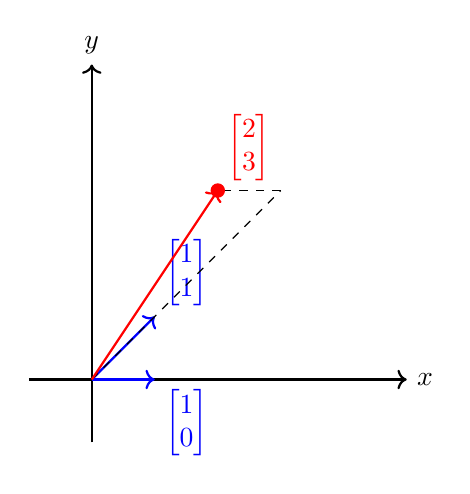
\begin{tikzpicture}[scale=0.8]
    % Axes
    \draw[->, thick] (-1, 0) -- (5, 0) node[right] {$x$};
    \draw[->, thick] (0, -1) -- (0, 5) node[above] {$y$};

    % Basis vectors
    \draw[->, thick, blue] (0,0) -- (1,1) node[above right] {$\begin{bmatrix}1\\1\end{bmatrix}$};
    \draw[->, thick, blue] (0,0) -- (1,0) node[below right] {$\begin{bmatrix}1\\0\end{bmatrix}$};

    % Step 1: 3*[1;1] = (3,3)
    \draw[dashed] (0,0) -- (3,3);

    % Step 2: -1*[1;0] = (-1,0) so (3,3)+(-1,0) = (2,3)
    \draw[dashed] (3,3) -- (2,3);

    % Final point
    \filldraw[red] (2,3) circle (3pt) node[above right] {$\begin{bmatrix}2\\3\end{bmatrix}$};

    % Coordinate arrow from origin to final point
    \draw[->, thick, red] (0,0) -- (2,3);
\end{tikzpicture}
\end{center}
\\
\newline
{For an $n$-dimensional vector space $V$ and an ordered basis $B$ of $V$, the mapping.}
$$
\phi: \mathbb{R}^n \to V, \quad \phi(e_i) = \vec{b}_i, \quad i \in \{1, \ldots, n\}
$$
is linear, where $(\vec{e}_1, \ldots, \vec{e}_n)$ is the standard basis of $\mathbb{R}^n$.
\\
\newline
{Transformation Matrix:} Let $V$, $W$ be vector spaces with ordered bases $\mathcal{B} \in B = (\vec{b}_1, \ldots, \vec{b}_n)$ and $\mathcal{C} = C = (\vec{c}_1, \ldots, \vec{c}_m)$ respectively.
\\
and consider a linear mapping:
$
\Phi : V \longrightarrow W.
$
For $j \in \{1, \ldots, n\}$, we have $\Phi(\vec{b}_j) \in W$. That is:
$$
\Phi(\vec{b}_j) = \alpha_{1j} \vec{c}_1 + \cdots + \alpha_{mj} \vec{c}_m = \sum_{i=1}^{m} \alpha_{ij} \vec{c}_i.
$$
\\
\newline
And this is a unique representation of $\Phi(\vec{b}_j)$. We define an $m \times n$ matrix $A_\Phi$ such that:
$$
A_\Phi(i,j) = \alpha_{ij}
$$
as the transformation matrix of $\Phi$ (with respect to the ordered bases $\mathcal{B}$ of $V$ and $\mathcal{C}$ of $W$).
\newpage
The coordinates of $\Phi(\vec{b}_j)$ lie in the $j^{\text{th}}$ column of $A_\Phi$. \\
Now, consider two finite-dimensional vector spaces $V, W$ with ordered bases $B, C$ and a linear mapping $\Phi : V \to W$ with transformation matrix $A_\Phi$. \\
\\
Let $\hat{x}$ be the coordinates of $\vec{x} \in V$ with respect to the ordered basis $B$.
$$\therefore
\vec{x} = B \hat{x}.
$$
Let $\hat{y}$ be the coordinate of $\phi(\vec{x}) \in W$ with respect to the ordered basis $C$. Therefore, 
$$
\phi(\vec{x}) = C \hat{y}.
$$

$$
C \hat{y} = \phi(\vec{x}) = \phi(B \hat{x}) = \phi\left(\hat{x}_1 \vec{b}_1 + \hat{x}_2 \vec{b}_2 + \dots + \hat{x}_n \vec{b}_n\right)
$$

$$
= \hat{x}_1 \phi(\vec{b}_1) + \hat{x}_2 \phi(\vec{b}_2) + \dots + \hat{x}_n \phi(\vec{b}_n)
$$

\begin{equation}
= \begin{bmatrix}
\phi(\vec{b}_1) & \phi(\vec{b}_2) & \dots & \phi(\vec{b}_n)
\end{bmatrix}
\begin{bmatrix}
\hat{x}_1 \\
\vdots \\
\hat{x}_n
\end{bmatrix}
\end{equation}


Here, we have assumed that, 
$
\hat{x} = 
\begin{bmatrix}
\hat{x}_1 \\
\vdots \\
\hat{x}_n
\end{bmatrix}
$
\\
$\because
\text{co-ordinates of } \phi(\vec{b}_j) \text{ is the } j^{\text{th}} \text{ column of } A_\phi \text{ in vector space } W \text{ w.r.t. ordered basis } C.
$\\
$$
\therefore \phi(\vec{b}_j) = C \, A_\phi(i,j)
\quad \left( A_\phi(i,j) \text{ shows the entire } j^{\text{th}} \text{ column of } A_\phi \right)
$$

$$
\implies 
\begin{bmatrix}
\phi(\vec{b}_1) & \dots & \phi(\vec{b}_n)
\end{bmatrix}
= C A_\phi
$$

Therefore, equation (1) can be written as:

$$
C \hat{y} = C A_\phi \hat{x}
$$\\
Since \( C \) has linearly independent columns (coordinates are unique),

\[
\therefore \hat{y} = A_\phi \hat{x}
\]
\\
Hence, \( A_\phi \) can be used as a mapping from the coordinates of \( \vec{x} \) with respect to basis \( B \) to coordinates of \( \phi(\vec{x}) \) with respect to basis \( C \).
\newpage
Consider a homomorphism (linear mapping), \(\phi: V \to W\) and ordered bases
$$
B = (\vec{b}_1, \vec{b}_2, \vec{b}_3) \quad \text{of } V \quad \text{and} \quad C = (\vec{c}_1, \vec{c}_2, \vec{c}_3, \vec{c}_4)  \text{ of }W \text{ with}
$$

\[
\begin{aligned}
\phi(\vec{b}_1) &= \vec{c}_1 - \vec{c}_2 + 3\vec{c}_3 - \vec{c}_4 \\
\phi(\vec{b}_2) &= 2\vec{c}_1 + \vec{c}_2 + 7\vec{c}_3 + 2\vec{c}_4 \\
\phi(\vec{b}_3) &= 3\vec{c}_2 + \vec{c}_3 + 4\vec{c}_4
\end{aligned}
\]

$$
A_\phi =
\begin{bmatrix}
1 & 2 & 0 \\
-1 & 1 & 3 \\
3 & 7 & 1 \\
-1 & 2 & 4
\end{bmatrix}
$$
\\
The transformation matrix \( A_\phi \) with respect to \( B \) and \( C \) satisfies \( \phi(\vec{b}_k) \).

Matrix:
$
R_{45^\circ} = \begin{bmatrix}
\frac{1}{\sqrt{2}} & -\frac{1}{\sqrt{2}} \\
\frac{1}{\sqrt{2}} & \frac{1}{\sqrt{2}}
\end{bmatrix}
\quad \text{rotates any vector by } 45^\circ
$\\
\newline
Transformation:
$
T = \begin{bmatrix}
2 & 0 \\
0 & 1
\end{bmatrix}
\quad \text{scales the vector's } x \text{ component to its double \\while keeping } y \text{ component as it is}.
$
\newline
\\
\textbf{Exercise:} Make a triangle in graphics, multiply all its coordinates with the given matrix \( R_{45^\circ} \). You will find that it will rotate the whole triangle by \( 45^\circ \) about the origin.
\end{document}


